\chapter{SafeGuard System}
\label{chapter:implementation}

\newenvironment{implementation}
{\quote\itshape}
{\endquote}

\begin{implementation}
    In this chapter, the SafeGuard implementation architecture is described, detailing each component and the 
    technology stack utilized, providing a comprehensive overview of how all parts of the system are 
    integrated and work together.
\end{implementation}

\section{Architecture Overview}
\begin{figure}[h]
    \centering 
    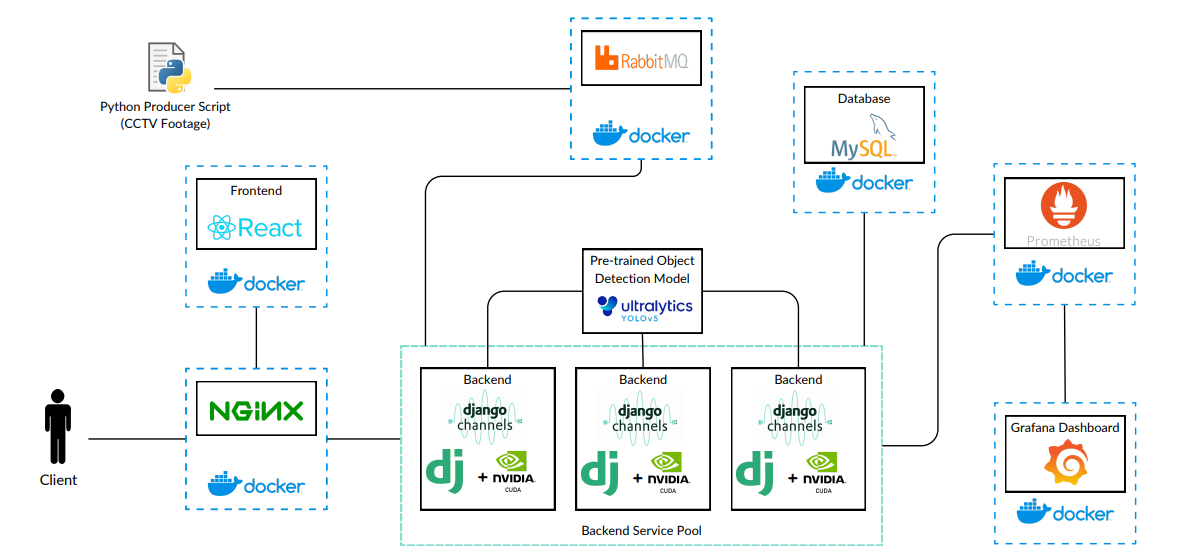
\includegraphics[width=0.95\textwidth]{figs/implementation-architecture6.png} 
    \caption{Implementation Architecture Overview}
    \label{fig:implementation-arch}
\end{figure}
Building this weapon detection system architecture, described in figure \ref{fig:implementation-arch},
 raises several challenges, 
especially integrating a trained model that detects weapons in real time enviroment,
and its large-scale deployment.

First, we developed a Python 3.10 script that simulates the CCTV footage, acting as a producer by sending video 
frames to the next stage (Queue Management), reproducing real-time surveillance.
Because we are dealing with various cameras with different video streams, the Queue Management was built under 
the RabbitMQ \cite{rfc48}, as message broker, which allows to organize video streams into queues
specific to each user, containing the video streams from their respective cameras. This
structure not only helps in managing the video data efficiently but also ensures that each
user's data is handled securely and separately.

The backend of the system is built using Django 5.0.6, chosen for its rapid development and maintainability, 
and employs \ac{gpu}/\ac{cuda} technology to enhance the 
running of detection model inference, a pre-trained \ac{yolo}v5 object detection model, fine-tuned with multiple
hyperparameters.
This component consumes the video data queued in RabbitMQ, 
processing each frame. Acting as the system's backbone, it coordinates both video processing and user 
management. Additionally, it supports user authentication and CRUD (Create, Read, Update, Delete) operations, 
interacting with a MySQL database essential for storing and managing user data and detection logs.

An essential feature of the system is its ability to detect weapons in the video frames. Upon detection, the backend 
uses Django Channels and WebSockets to trigger real-time alerts. These alerts are instantly pushed to the frontend, 
ensuring immediate user notification, which is crucial for prompt response and intervention in 
security-sensitive situations.

To manage client requests efficiently, Nginx, known for its speed and efficiency, has been deployed as a load balancer, 
distributing requests evenly among three backend services.
Each backend service shares the pre-trained model, ensuring consistency and reliability in detection results. 
Nginx's lightweight design minimizes its resource usage, allowing the system to run smoothly, ensuring high 
availability and improved performance of the system.

%The user interface is developed using React 18.0.2 designed to be intuitive and user-friendly, providing users with 
%real-time alerts from the backend, a dedicated page listing all cameras associated with them, and a historical log 
%of all detections. Additionally, there is an upload page where users can analyze past recorded videos.

The user interface is built with React 18.0.2, influenced by the familiarity with React for creating user-friendly web 
apps and also for its flexibility. The interface, designed to be intuitive and user-friendly, 
provides real-time alerts from the backend, a dedicated page listing 
all associated cameras, and a historical log of detections. Additionally, there's an upload page for analyzing past 
recorded videos.

Furthermore, Prometheus and Grafana have been integrated for monitoring and visualization of system performance metrics.
This duo provides a clear picture of how the system is running, allowing for proactive maintenance and real-time 
tracking of system health.  Prometheus collects data on various aspects of the system's performance, and Grafana 
transforms this data into easy-to-understand charts and graphs.

\section{Folder Structure}
This section outlines the structure of the project directories and files, designed to support a modular and 
scalable application, figure \ref{fig:folder-structure}.

The root directory, \textit{project/}, serves as the central hub containing all the subdirectories and 
configuration files pertinent to the project. It includes:
\begin{itemize}
    \item Nginx configuration file
    \item Docker configuration file
    \item Producer script
    \item Backend folder
    \item Frontend folder
\end{itemize}

The \textit{backend/} directory of the project has the server-side logic, developed using the Django framework. 
This setup includes all necessary components of a Django application, including models, views, and 
controllers. These elements handle the business logic and database operations and are located within the \textit{base/} 
folder.
The directory also
contains a \textit{requirements.txt} file, 
crucial for defining all the Python dependencies required for the backend. Additionally, it includes the detection 
model files.

In contrast, the \textit{frontend/} directory focuses on the client-side elements of the application, utilizing React to 
build the user interface. This directory contains the main React components and views. It also includes a 
Dockerfile, which specifies how to build the
Docker container for the React application. 
The components/ subdirectory holds individual javascript files that define specific parts of the user interface.

\begin{figure}[h]
    \centering 
    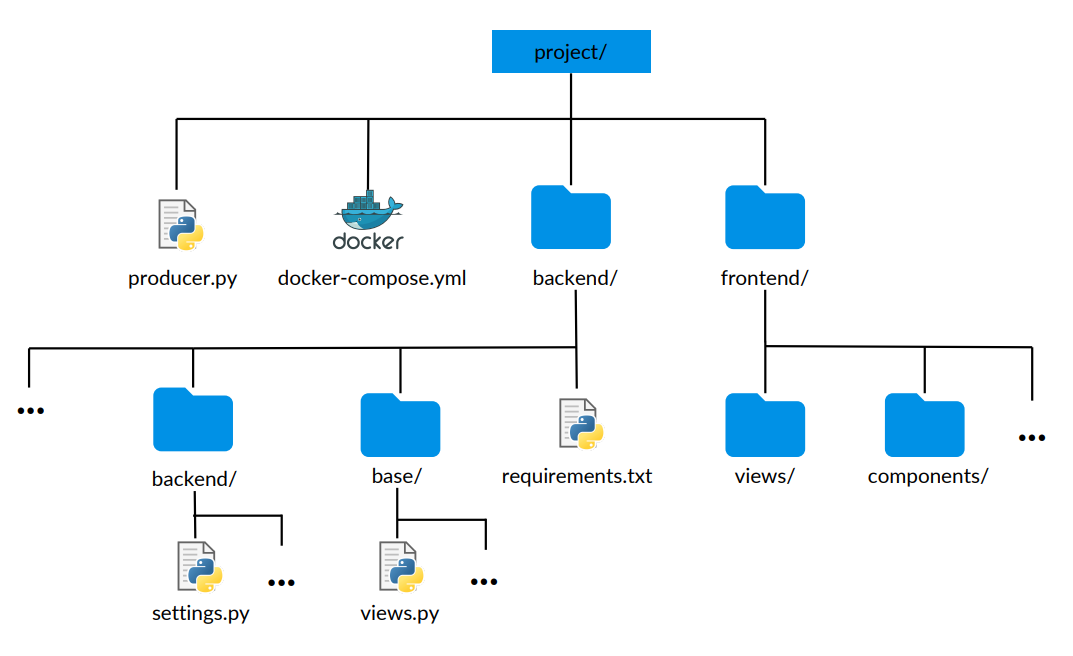
\includegraphics[width=0.7\textwidth]{figs/folder.png} 
    \caption{Folder Structure Diagram}
    \label{fig:folder-structure}
\end{figure}

\section{Video Retrieval and Management}
\subsection{RabbitMQ Setup}
RabbitMQ is a widely adopted message broker that efficiently manages messaging and streaming, making it an ideal 
choice for applications that require robust and scalable message handling. It is 
designed for reliability and flexibility, easily deployed across cloud environments, on-premises, or locally, serving 
millions of users worldwide \cite{rfc48}. Its versatility and reliability make RabbitMQ a fitting backbone for our Django-React 
application, where it orchestrates video data streaming from simulated \ac{cctv} cameras.

To integrate RabbitMQ into our Django-React application, we employ Docker for containerization, which simplifies the 
deployment and scalability of services. The configuration of RabbitMQ within a Docker environment is specified in the 
docker-compose.yml file. Below, are outlined the key settings:
\begin{itemize}
    \item Image: 
        \begin{itemize}
            \item \textit{rabbitmq:3-management} image is used, which includes the management plugin for easy monitoring and management through a web-based interface.
        \end{itemize}
    \item Environment Variables:
        \begin{itemize}
            \item \textit{RABBITMQ\_DEFAULT\_USER} sets the default username.
            \item \textit{RABBITMQ\_DEFAULT\_PASS} specifies the default password.
        \end{itemize}
    \item Ports:
        \begin{itemize}
            \item 5672 is exposed for RabbitMQ server connections.
            \item 15672 is exposed for accessing the RabbitMQ management interface.
        \end{itemize}
    \item Volumes:
        \begin{itemize}
            \item a dedicated volume, \textit{rabbitmq-data}, is used to persist RabbitMQ data and configurations, ensuring data durability across container restarts.
        \end{itemize}
\end{itemize}


\subsection{Message Queuing and Processing}
The message queuing and processing subsystem is crucial for managing the flow of video data from \ac{cctv} cameras to 
the processing backend efficiently, as illustrated in picture \ref{fig:rabbit-mq}. 

RabbitMQ operates by holding, temporarily, messages in queues until they can be safely processed by consumers. 
The setup process involves configuring RabbitMQ queues for each \ac{cctv} camera source. 
These queues store video frames that are encoded as Base64 strings and tagged with metadata: \textit{camera\_id}, 
\textit{user\_id} 
and \textit{timestamp}.

\begin{figure}[h]
    \centering 
    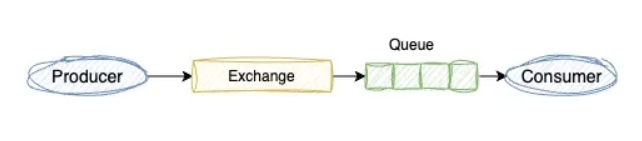
\includegraphics[width=0.5\textwidth]{figs/rabbitmq.png} 
    \caption{RabbitMQ~\cite{rfc48}}
    \label{fig:rabbit-mq}
\end{figure}

The process initiates with each video file from the \ac{cctv} camera being processed frame by 
frame. The OpenCV library \cite{rfc59} is used to capture video frames, which are then encoded into a JPEG format using base64 to 
facilitate easy transmission over the network. Each frame is packaged into a JSON object containing relevant metadata 
and pushed to the designated RabbitMQ queue.

The key function \textit{send\_frame\_to\_queue} is responsible for publishing each frame to its respective queue. 
It constructs a message payload containing the encoded frame and metadata, then sends
this message to the RabbitMQ exchange with a specific routing key corresponding to the queue name.

To enhance the throughput and responsiveness of the system, the video processing operation is executed in multiple 
threads. Each thread handles a different video source, allowing the system to parallelize the workload effectively.
\section{Frontend Development}
\subsection{Views Implementation}
After authentication, user is presented with the first view which lists all the cameras 
associated with their account, as showed in figure \ref{fig:camera-list}. This ensures that users have organized access to 
their specific surveillance resources. 

As mentioned above, the system uses RabbitMQ, which maintains a queue dedicated to each user. When cameras stream video, 
RabbitMQ receives these frames and forwards them to the backend. 
From there, the backend processes these 
frames and sends them to the frontend via WebSockets.

Upon selecting a camera, the user is directed to a second view where the video footage is streamed live, as illustrated in
 figure \ref{fig:camera-page}. 
In parallel, the stream is analyzed using an object detection model. The details of this model, which will be discussed 
subsequently, include the identification of specific objects of interest, in this instance, weapons.

When a weapon is detected, the system triggers an alert that is immediately relayed to the user through a toaster 
notification on the frontend interface. This alert specifies the type of weapon detected and the confidence level 
of the detection, providing information immediately to the user. 

Furthermore, the system ensures that all detections are recorded in a database in real time, thus providing a 
comprehensive and accurate record of events.
This ability to retain data indefinitely permits retrospective analysis, which can prove 
instrumental in both investigative and monitoring activities.

\begin{figure}[h]
    \centering
    \begin{subfigure}[b]{0.49\textwidth}
        \centering
        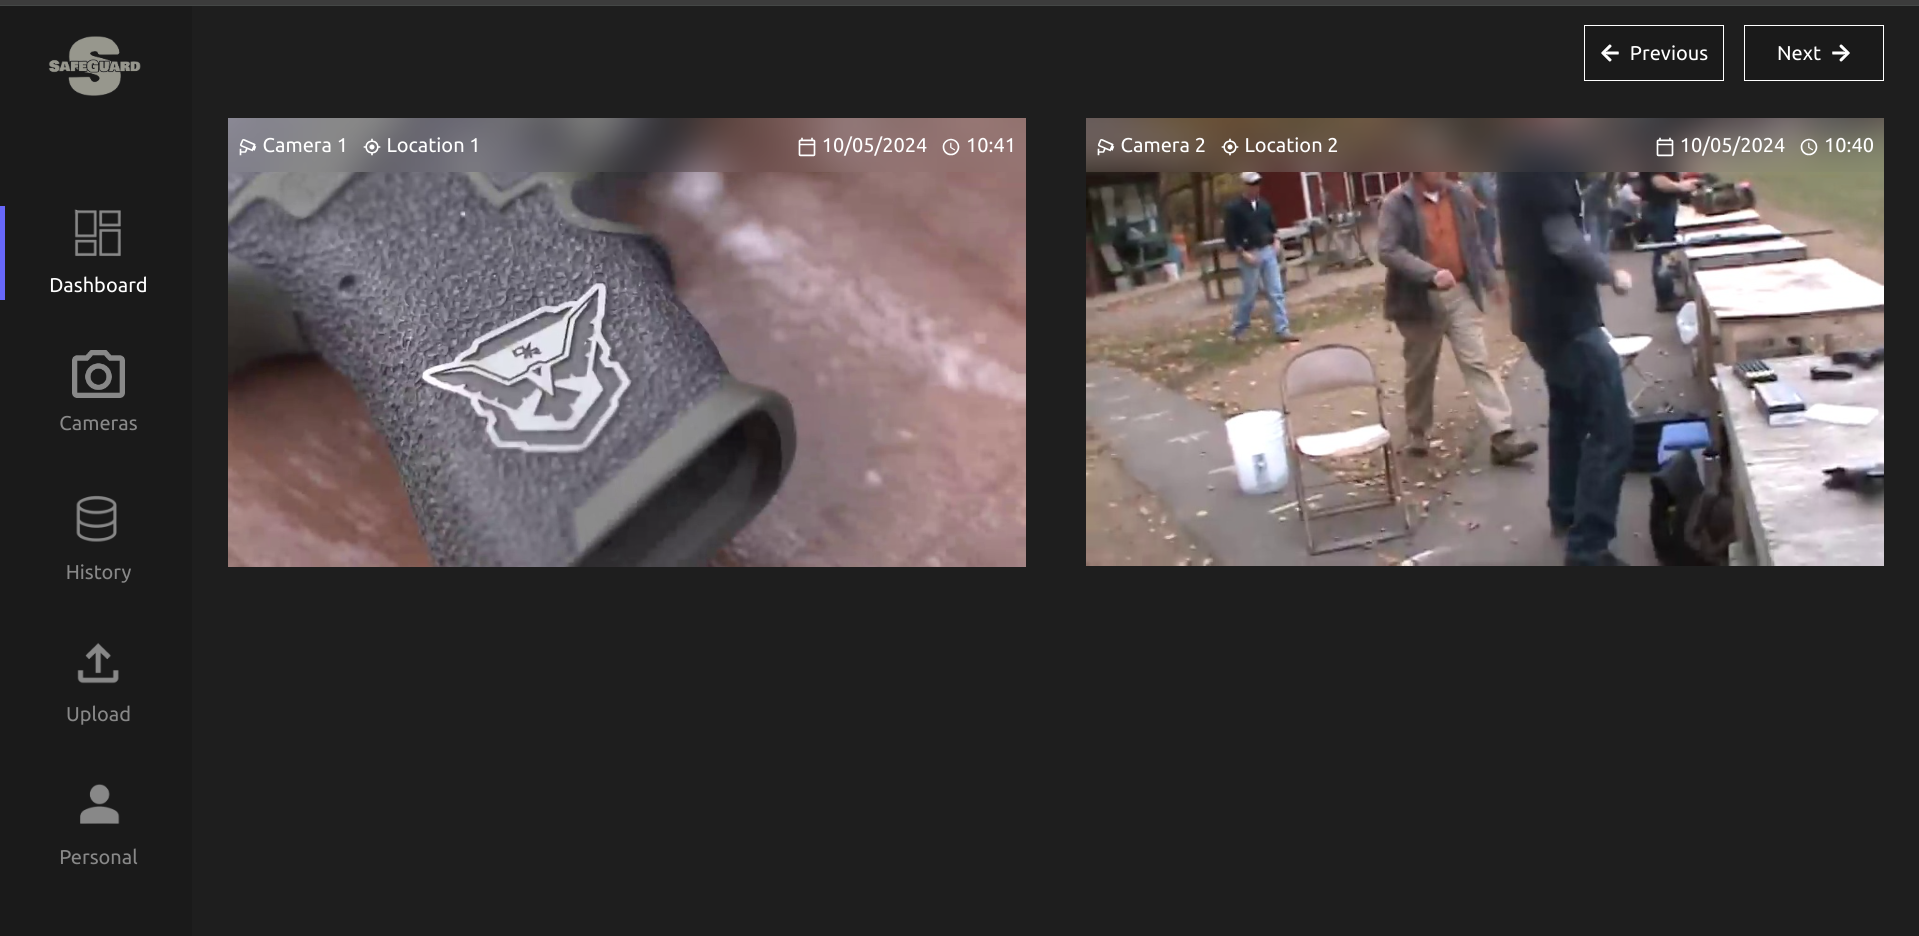
\includegraphics[width=\linewidth]{figs/cameras-list.png}
        \caption{User Listed Cameras}
        \label{fig:camera-list}
    \end{subfigure}
    \hfill % spacing
    \begin{subfigure}[b]{0.49\textwidth}
        \centering
        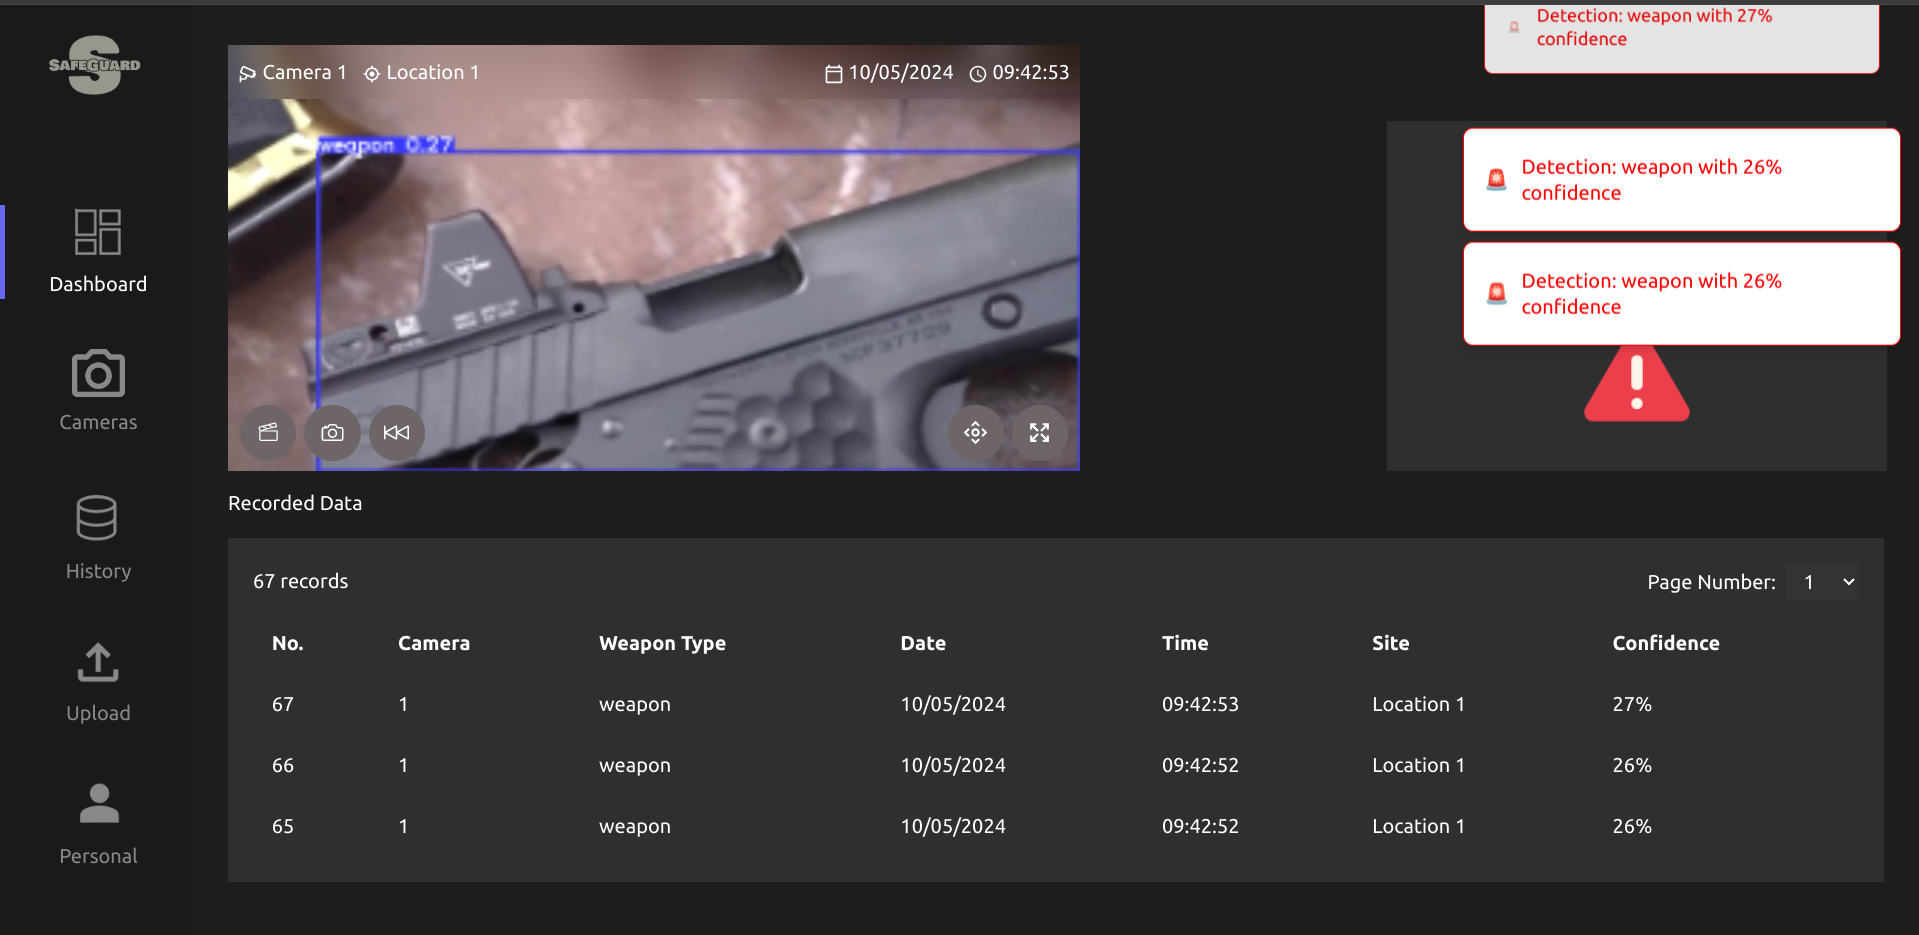
\includegraphics[width=\linewidth]{figs/camera-page.png}
        \caption{Single Camera Analysis}
        \label{fig:camera-page}
    \end{subfigure}
    \caption{Single and Multi Camera Pages}
    \label{fig:cameras-list-camera-analysis}
\end{figure}

Users may access the aforementioned historical data through a History page, as ilustrated 
in Figure \ref{fig:detections-history}, where 
they can view specific instances of detected weapons, including the time of detection and the captured frame.
\begin{figure}[h]
    \centering 
    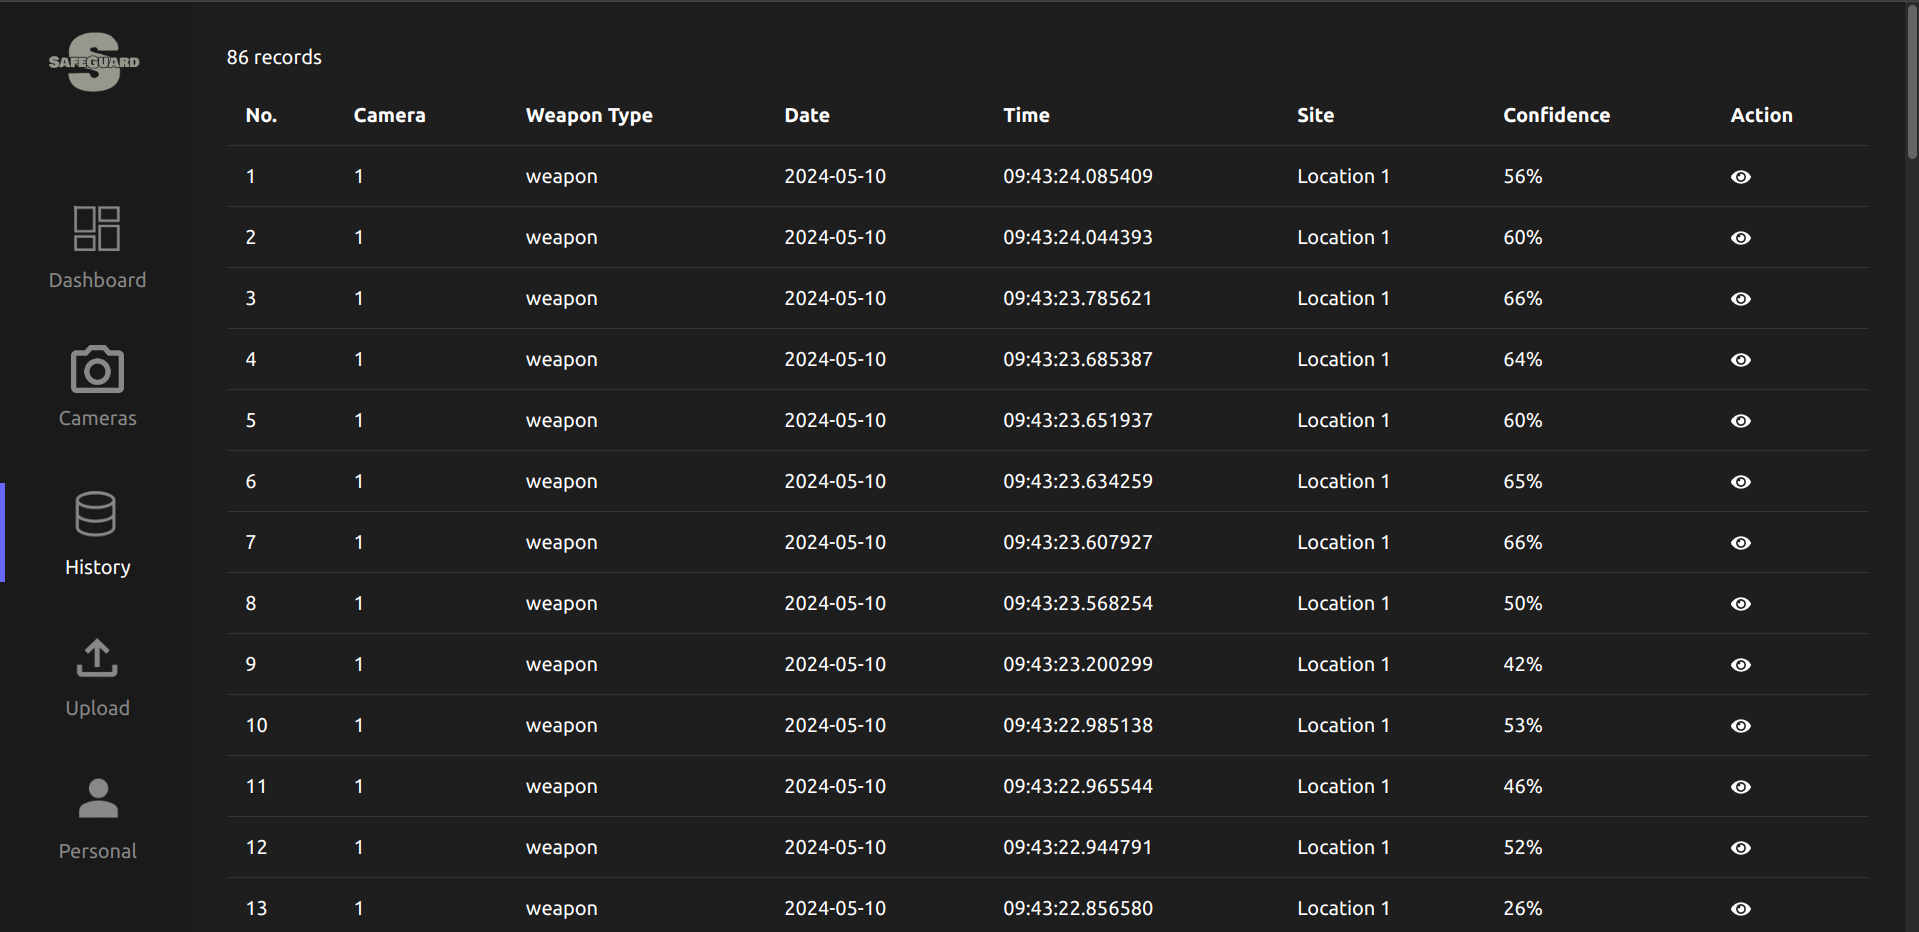
\includegraphics[width=0.65\textwidth]{figs/history-page.png} 
    \caption{Detections History Page}
    \label{fig:detections-history}
\end{figure} 

The application includes a section dedicated to the analysis of pre-recorded videos. This section 
allows users to select and upload a video file in the .mp4 format. %as illustrated in figure \ref{fig:upload-video}.

%\begin{figure}[h]
%    \centering 
%    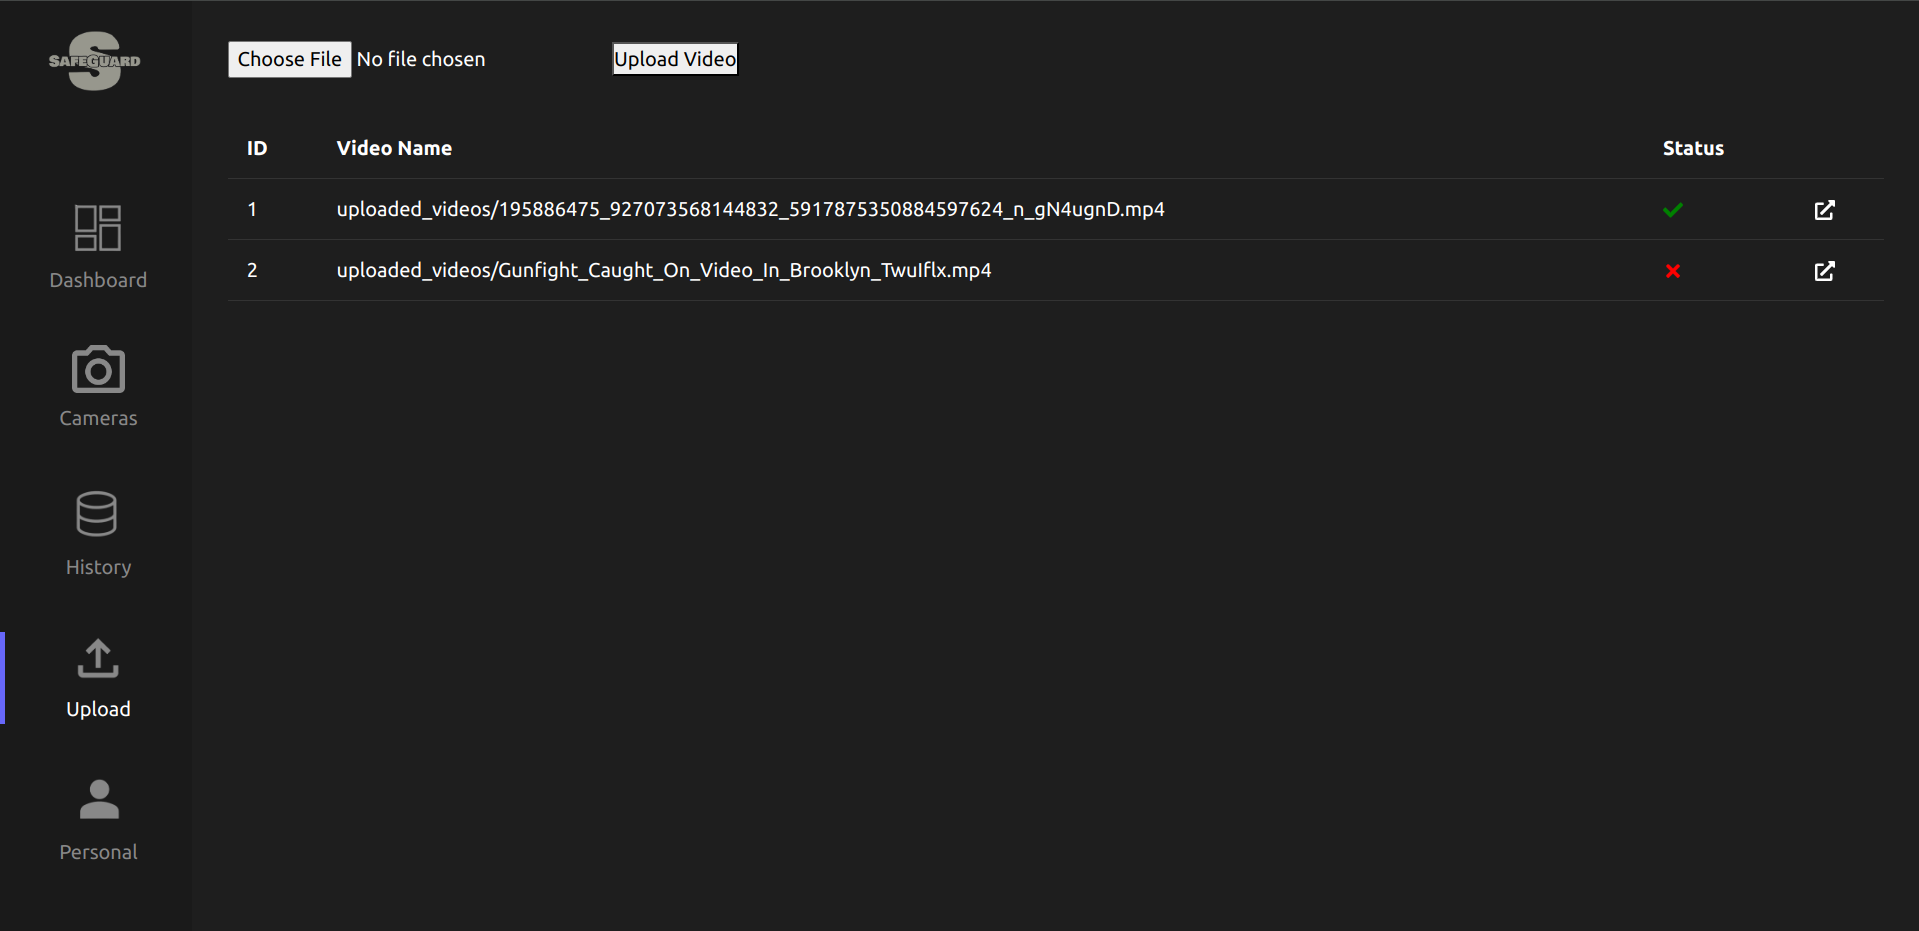
\includegraphics[width=0.65\textwidth]{figs/upload-video-page.png} 
%    \caption{Upload Video File}
%    \label{fig:upload-video}
%\end{figure}

Once a file is uploaded, it appears in a specific list that displays all of the files they have submitted, providing 
users quick access to their uploaded content and enabling them to track the status of each video.

Each file in the list is followed by a status indicator. If a video has not yet been analyzed, its status 
will reflect this, and selecting the video will lead the user to a page where the analysis process begins afresh, 
as ilustrated in figure \ref{fig:upload-video-analysis}. 
Importantly, any previous detections associated with the video are cleared to ensure that the analysis starts from 
the beginning, providing a clean slate for accurate detection. The analysis must run to the completion of the video 
for it to be marked with a check, signifying that it has been fully processed.

For videos that have already been analyzed, users can immediately access and download the processed video, \ref{fig:download-video}. 
The video version presented here includes bounding boxes, drawn around the weapons identified by the system, which 
visually indicate the location and presence of potential threats within the footage. 
Alongside the video, a list of detections are provided in a detailed table. 
This table includes the type of weapon detected, confidence score and the exact timestamp within the video where each 
weapon appears.

\begin{figure}[h]
    \centering
    \begin{subfigure}[b]{0.49\textwidth}
        \centering
        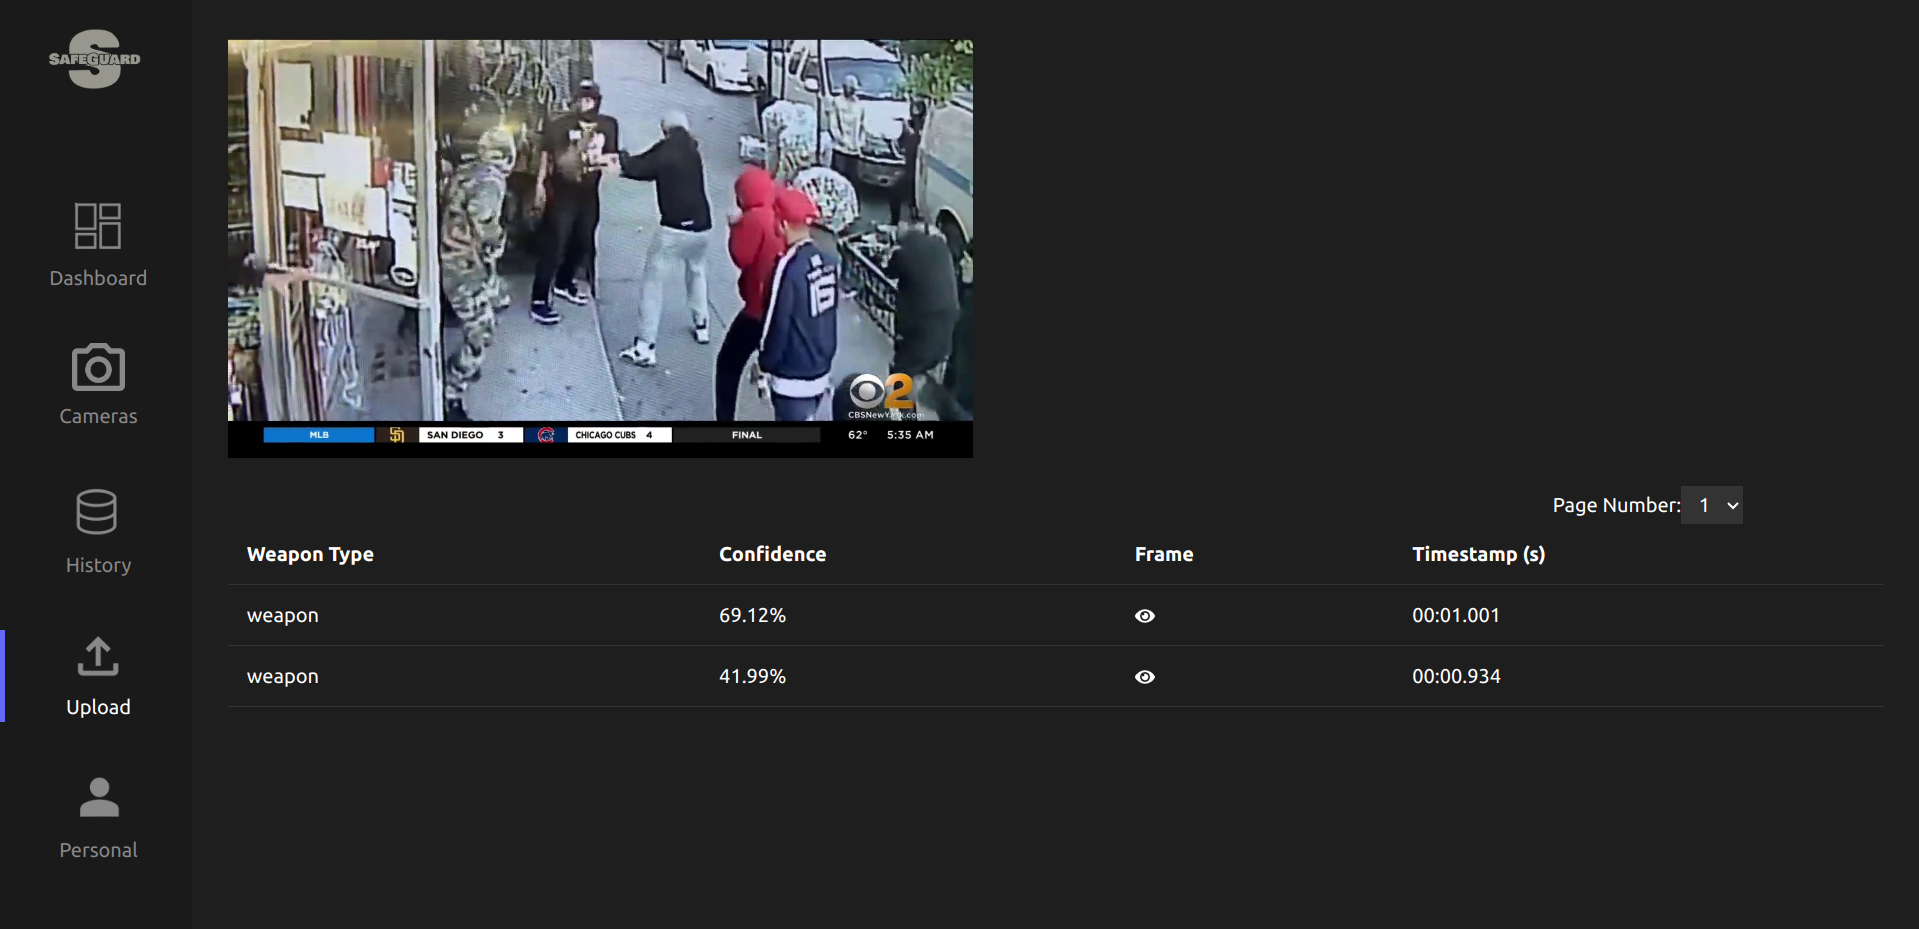
\includegraphics[width=\linewidth]{figs/video-upload-analysis-page.png}
        \caption{Upload Video Analysis}
        \label{fig:upload-video-analysis}
    \end{subfigure}
    \hfill % spacing
    \begin{subfigure}[b]{0.49\textwidth}
        \centering
        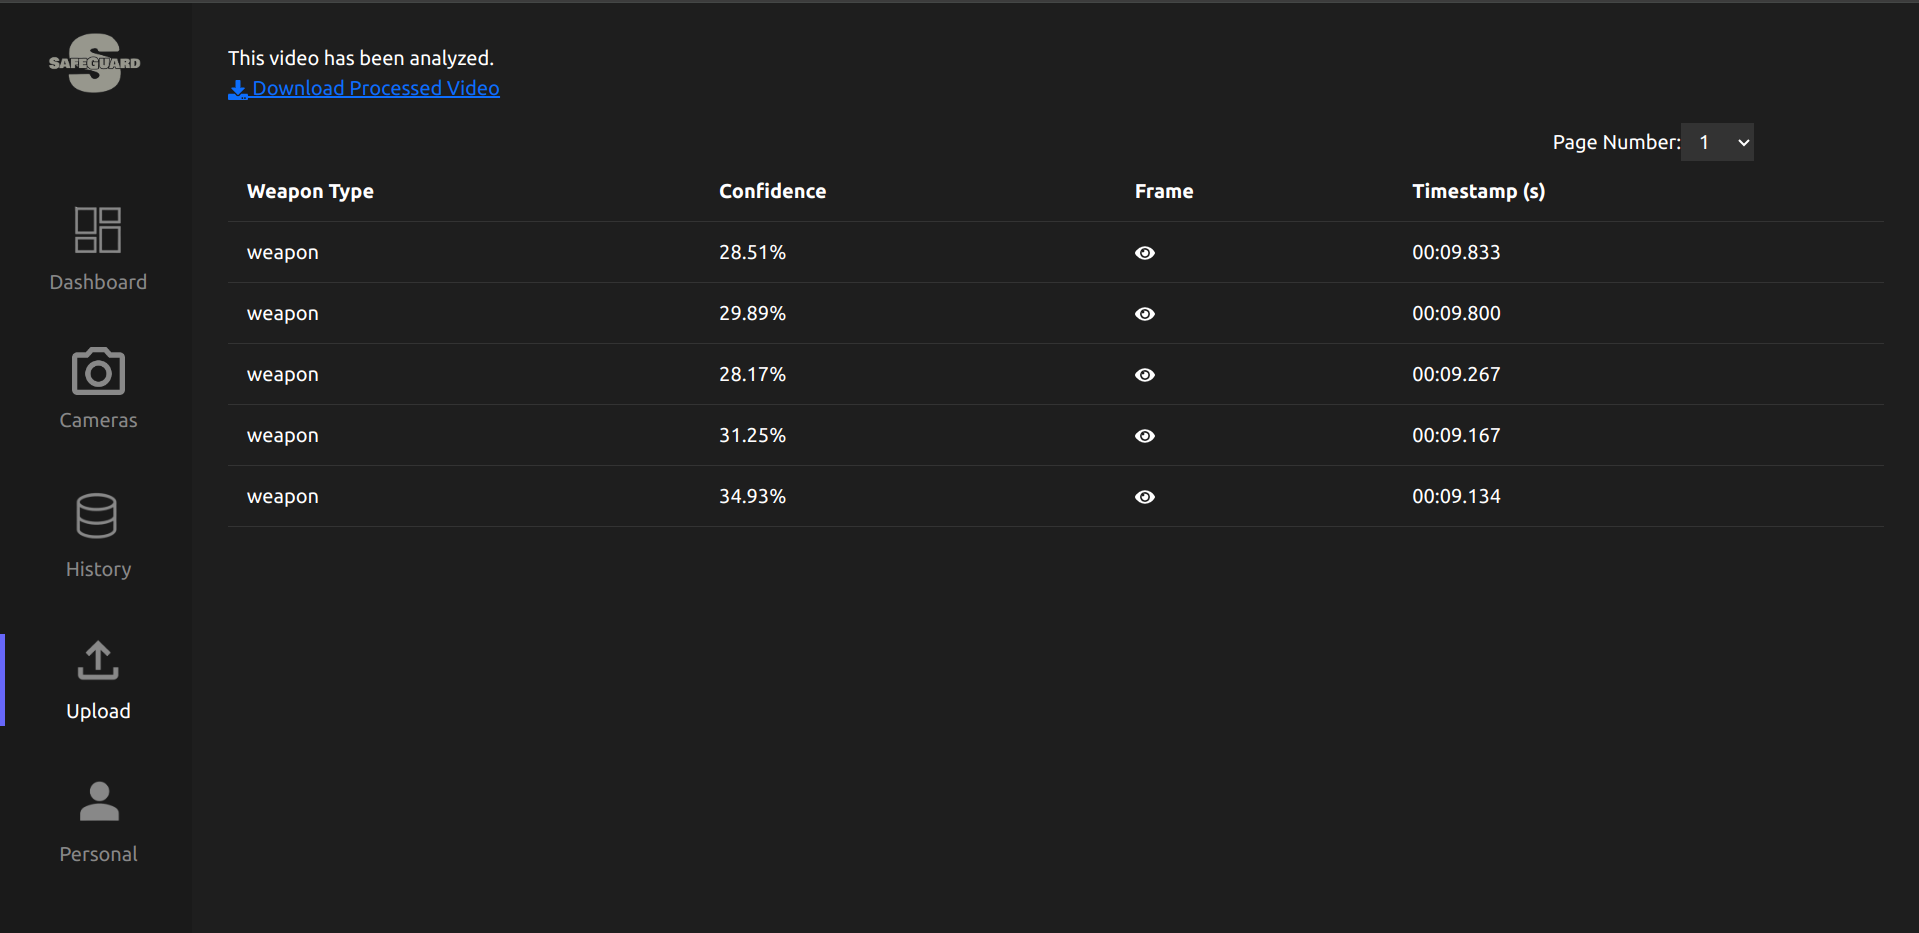
\includegraphics[width=\linewidth]{figs/download-video-page.png}
        \caption{Download Video after Analysis}
        \label{fig:download-video}
    \end{subfigure}
    \caption{Upload Video Feature}
    \label{fig:upload-video-section}
\end{figure}
\subsection{Integration with Docker}
By using Docker, the frontend is encapsulated in a controlled, consistent environment, ensuring that all 
dependencies and configurations are unified across different development and production stages.

The frontend service is built using a Dockerfile 
\footnote{\url{https://github.com/pedromonteiro01/cctv-real-time-weapon-detection/blob/main/project/frontend/Dockerfile}} 
that specifies \textit{node:alpine} as the base image. 
The service configuration includes essential commands to set up the 
working environment, install dependencies, and prepare the service to be run with the \textit{yarn start} command. 
Specifically, the \textit{COPY} commands transfer the necessary project files into the container, and the \textit{RUN} 
command installs all node modules as specified in \textit{yarn.lock}.

This setup facilitates a more efficient development process, allowing for rapid testing and deployment while maintaining 
high reliability and compatibility across various environments. Additionally, the direct transfer of project files 
and dependency management through Docker ensures that the application behaves predictably in every run, reducing 
potential deployment issues.
\subsection{Testing and Quality Assurance}

In frontend development, testing is a critical component that ensures the application is reliable, 
user-friendly, and robust. Three main types of testing have been implemented: unit tests, integration tests, 
and \ac{e2e} tests.

%\begin{figure}[h]
%    \centering 
%    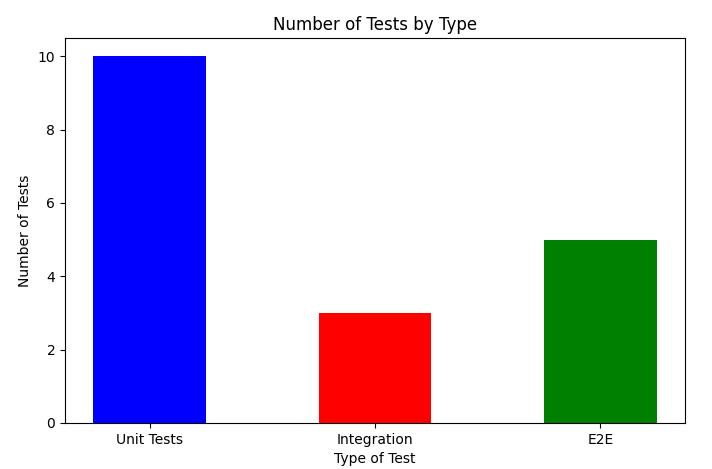
\includegraphics[width=0.5\textwidth]{figs/frontend-tests.png} 
%    \caption{Frontend Types of Tests}
%    \label{fig:frontend-tests}
%\end{figure}

The unit tests were developed using Jest \cite{rfc60} with the main objective to test individual components in isolation. 
This approach focused on ensuring the correct functionality of each component, examining internal logic, state 
management, and behavior under various conditions.

Integration tests were also conducted using Jest. These tests are crucial for assessing the interactions between 
connected components and services. The focus here was on the data flow and state management across components.

For \ac{e2e} testing, was used Selenium \cite{rfc61} with the Firefox driver \cite{rfc62} to simulate real user interactions from start to finish. 
This testing ensures the system behaves as expected in a production-like environment and includes several specific 
scenarios:

\begin{itemize}
    \item Login Test: ensured that authentication works correctly 
    and the user gains access to their account (code listing \ref{lbl:login-test-code});
    \item Upload Video File for Detection: tested the upload of a video file for 
    analysis, ensuring the application handles file uploads and data processing accurately;
    \item Download Analysed Video File: ensures users can download the processed video files, 
    confirming that the files are accessible;
    \item Get User Cameras List: verify that the application could correctly interact with the backend to 
    display the list of the user's connected cameras.
\end{itemize}

Below is an excerpt of the login test, code listing \ref{lbl:login-test-code}.

\begin{listing}[h]
    \begin{minted}{python}
    try:
        driver.get('http://localhost:3000/login') 
        driver.find_element(By.NAME, "username").send_keys("pmapm@ua.pt")
        driver.find_element(By.NAME, "password").send_keys("password")
        driver.find_element(By.CSS_SELECTOR, "button[type='submit']").click()

        time.sleep(5)

        if driver.current_url == 'http://localhost:3000/personal':
            print("Login successful")
        else:
            print("Login failed")
    finally:
        driver.quit()
    \end{minted}
    \caption{Login Test.}
    \label{lbl:login-test-code}
    \end{listing}

The login test navigates to the login page, inputs the 
username "pmapm@ua.pt" and 
password "password", and submits the form. After waiting for 5 seconds, it checks if the URL is 
http://localhost:3000/personal to verify if the login was successful. Finally, it closes the web driver.


\section{Backend Development}
\subsection{Authentication and Security}
This section explores the authentication and security mechanisms implemented in the backend. 
To manage the users of the application, a custom user model was defined, having key attributes such as email, 
names, and password. 

\begin{figure}[h]
    \centering 
    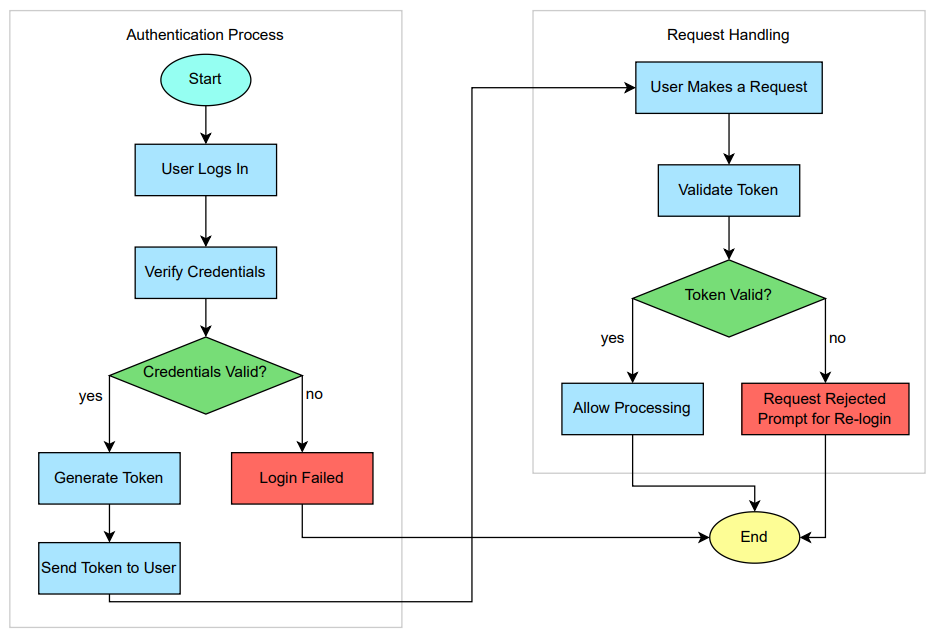
\includegraphics[width=0.75\textwidth]{figs/flow-chart.png} 
    \caption{Authentication Flowchart}
    \label{fig:auth-flowchart}
\end{figure}

Following the flowchart \ref{fig:auth-flowchart}, when a user successfully logs into the system using their credentials (email and password), the backend 
verifies these credentials against the stored data. If the credentials are correct, the server generates a token. 
This token acts as a stand-in for the user's credentials during future requests, thus avoiding the need to resend 
the password over the network, which could be intercepted. Each token is unique and tied specifically to one user.

Once the token is generated and sent back to the user's client, a web browser, it is stored locally, in local storage. 
Every subsequent request will include this token in the request headers, to tell the server which user is making 
the request.

Upon receiving a request that includes a token, the server first validates the token. This validation process checks 
if the token is valid, has not expired, and is linked to an actual user account. If any of these checks fail, 
the server will reject the request.

If the token is valid, the system allows to process the request coming from the user.

For added security, tokens are configured to expire after a certain period. This limits the time an attacker has to 
use a stolen token. When a token expires, the user must log in again, and a new token is generated.

\subsection{Client-Server Interaction Flows}
The system interactions between the client and server, described in figure \ref{fig:flows}, are divided 
into two main processes, each supporting a different aspect of video management and surveillance. 
\begin{figure}[h]
    \centering
    \begin{subfigure}[b]{0.45\textwidth}
        \centering
        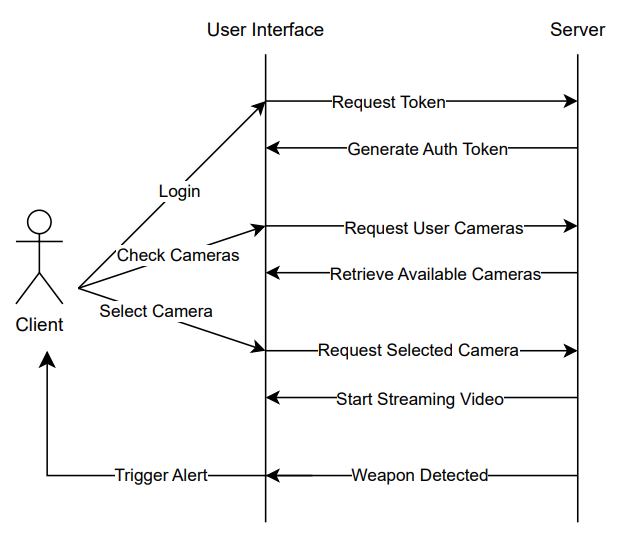
\includegraphics[width=\linewidth]{figs/flow1.png}
        \caption{Real-time Camera Detections Flow}
        \label{fig:flow1}
    \end{subfigure}
    \hfill % spacing
    \begin{subfigure}[b]{0.45\textwidth}
        \centering
        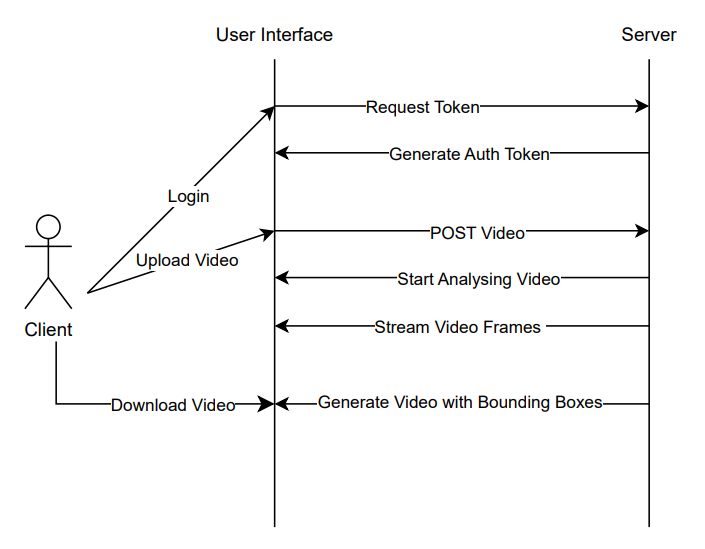
\includegraphics[width=\linewidth]{figs/flow2.png}
        \caption{Upload/Download Video Flow}
        \label{fig:flow2}
    \end{subfigure}
    \caption{Basic Client-Server Interaction Flows}
    \label{fig:flows}
\end{figure}

The \ref{fig:flow1} flow begins with the client logging into the system, establishing a secure session 
through user authentication. Following successful login, the client requests an authentication token, which the 
server generates and sends back. This token is crucial for validating the subsequent requests by the client under 
the secure session.

Once authenticated, the client requests access to the cameras associated with their account. The server responds by 
retrieving and sending a list of available cameras. The user selects a camera from this list, and the client sends a 
request to access the selected camera. The server, upon receiving this request, starts streaming video from the chosen 
camera directly to the client.

During the streaming, if the server's analysis algorithms detect a weapon in the video, it triggers an alert. 
This alert is then sent to the client, notifying them of the potential threat.

The second flow, \ref{fig:flow2}, also starts with the client logging in and obtaining an authentication token, ensuring a 
secure environment for data exchange. After login, the client uploads a video file for analysis, using a POST 
request. This video is selected from the user's local device and is sent to the server.

Upon receiving the video, the server initiates the analysis using a pre-trained object detection algorithm. 

After completing the analysis, the server generates a new version of the video, which is the output 
of the model, featuring bounding boxes around the detected objects. This annotated video is then made 
available for the client to download.

\subsection{Data Models}

In Django, models play a crucial role by serving as the structural foundation of the database. 
These models, represented in image \ref{fig:db-schema}, enable the seamless translation of database schemas into Django objects, facilitating CRUD 
(Create, Read, Update, Delete) operations through Python code, bypassing the need for direct SQL interaction.

\begin{figure}[h]
    \centering 
    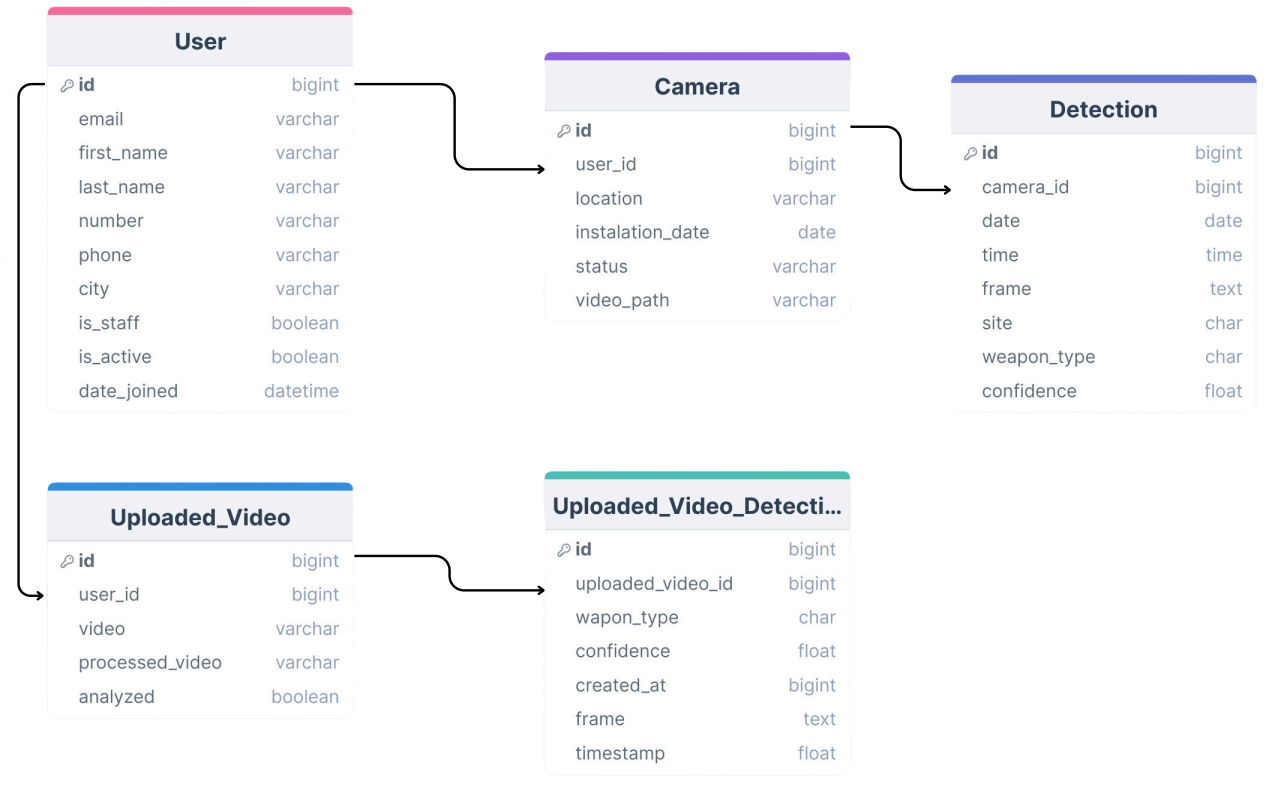
\includegraphics[width=0.8\textwidth]{figs/database-schema2.png} 
    \caption{Database Schema}
    \label{fig:db-schema}
\end{figure}

The User model at the core of this schema stores not only the credentials that officers use to access the application 
but also their personal information such as the name, contact number, and city of residence. This model also includes 
access control attributes, such as staff privileges, for managing 
permissions within the application.

Each police officer using the platform can manage multiple cameras. These cameras, detailed in the Camera model, 
are installed in various locations and are integral to capturing continuous video footage. The Detection model is 
essential for logging specific events detected by the cameras. It captures critical details such as the date, time, 
frame of detection, and the type of weapon detected, if any, along with the detection's confidence level. This 
information is vital not only for real-time alerts but also for historical data analysis, which is essential for 
post-event investigations.

Furthermore, the application supports an upload feature, allowing officers to upload video files for analysis. 
The Uploaded Video model maintains a direct association with the user, ensuring clear accountability for each 
video uploaded. It tracks whether each video has been analyzed, helping in the workflow management of video processing.

The Uploaded Video Detection model focus on detections within the uploaded videos. 
It records similar details as the Detection model, such as the type of weapon detected, the confidence level of 
the detection, and the specific frame and time within the video where the detection occurred.
\subsection{API Endpoints}
Views are a crucial component that handle the logic and control flow of applications by responding to requests from users.
Views interact with models and render appropriate responses, usually in the form of HTML pages, JSON, or XML, depending 
on the application's requirements.

The application is structured around three principal groups of endpoints, each dedicated to a specific aspect of 
the application's functionality: user management, detections, and uploaded videos. 

The first group of endpoints, \ref{fig:views-user}, focuses on user management, facilitating secure and straightforward user 
interactions with the application. The primary entry point is the login endpoint, where users authenticate by 
submitting their credentials. Successful authentication returns a session token, crucial for maintaining a 
secure and personalized session. Once authenticated, users can retrieve their profile information such as 
name, email, and role within the application.

\begin{figure}[h]
    \centering 
    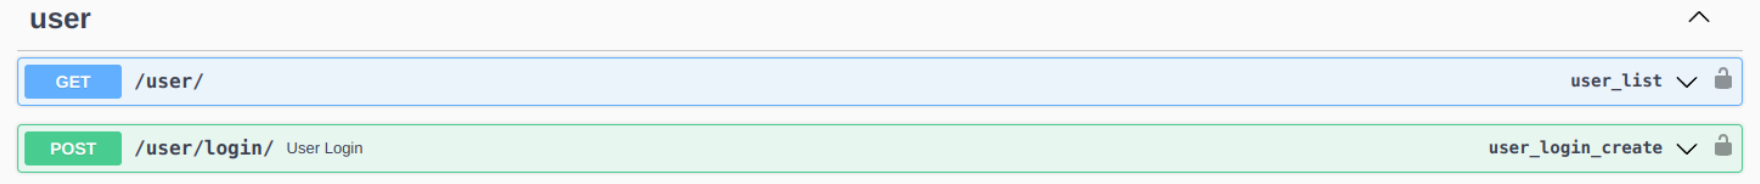
\includegraphics[width=0.95\textwidth]{figs/views-user.png} 
    \caption{User Views}
    \label{fig:views-user}
\end{figure}

Detections play a crucial role in the application, supporting both real-time security monitoring and 
historical data analysis. The POST /detections/ endpoint is designed for the application to 
submit new detection records to the database in real time when an incident is detected by a specific camera.

On the other hand, the GET method allows the application to retrieve all detection records for all cameras associated 
with a specific user. This endpoint is particularly helpful for creating a historical overview of detections,
which users can access to review and analyze past incidents.

\begin{figure}[h]
    \centering 
    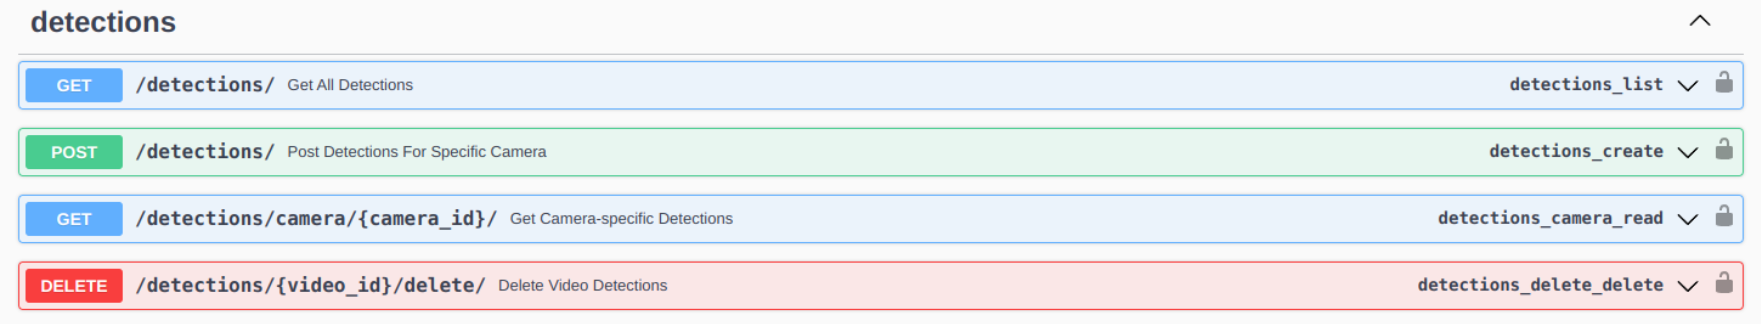
\includegraphics[width=0.95\textwidth]{figs/views-detections.png} 
    \caption{Detections Views}
    \label{fig:views-detections}
\end{figure}

Additionally, the application includes a DELETE endpoint, for the 
removal of detections associated with a particular video. This feature enables the management of stored detection data. 

The uploaded videos section of the application addresses the need to analyze previously recorded or 
externally sourced video footage. Users can upload videos through the upload video endpoint, which processes and 
stores the videos in the database, linking them to the user's account for secure and easy access.
\begin{figure}[h]
    \centering 
    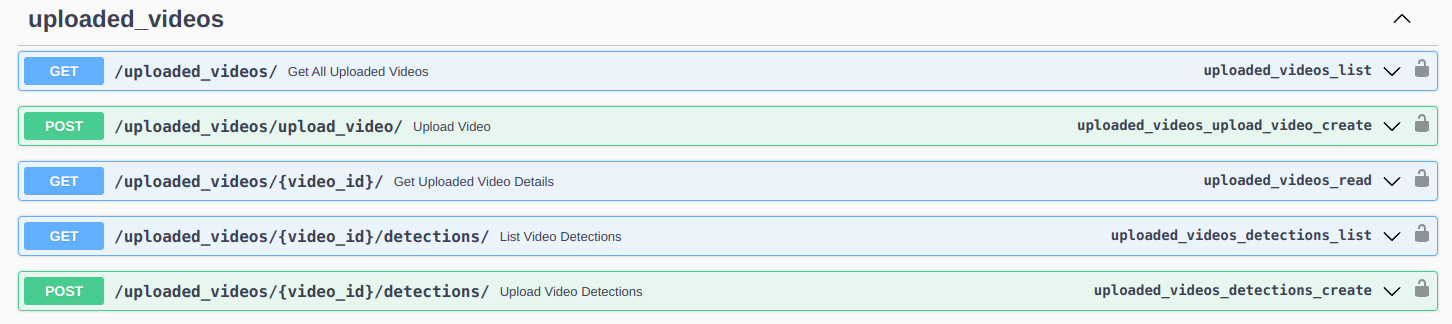
\includegraphics[width=0.95\textwidth]{figs/views-videos.png} 
    \caption{Uploaded Video Views}
    \label{fig:views-video}
\end{figure}

The application also includes a \textit{/metrics/} endpoint, which exposes Prometheus metrics using 
\textit{django\_prometheus}. This endpoint provides essential performance and operational metrics for the 
application, facilitating monitoring and alerting. These metrics cover a range of data points, such as request rates, 
response times, and error rates. This feature will be discussed in more detail in the subsequent sections.


\subsection{Django Consumers}
This section discusses the three distinct types of consumers used in the 
application: \textit{VideoStreamConsumer}, \textit{MultiCameraStreamConsumer}, and \textit{UploadedVideoStreamConsumer}.

The core of these consumers' operations begins with the initialization of the computational environment, 
specifically using \ac{gpu} acceleration via \ac{cuda} for real-time video analysis.

All consumers initiate their processing by setting up the necessary computational resources to ensure efficient 
video analysis. This setup involves determining the availability of a \ac{gpu} and utilizing 
\ac{cuda} (Compute Unified Device Architecture) for accelerated computing \ref{lbl:cuda-init}. DataParallel is used 
to distribute the model across multiple \ac{gpu}s if more than one \ac{gpu} is available.

\begin{listing}[h]
    \begin{minted}{python}
    device = "cuda" if torch.cuda.is_available() else "cpu"

    # load model and wrap it with DataParallel if multiple GPUs are available
    model = torch.hub.load('ultralytics/yolov5', 'custom', path='base/best.pt').to(device)
    if torch.cuda.device_count() > 1:
        print(f"Using {torch.cuda.device_count()} GPUs!")
        model = DataParallel(model)
    \end{minted}
    \caption{Cuda Initialization.}
    \label{lbl:cuda-init}
    \end{listing}

The \textit{VideoStreamConsumer} is fitted for handling real-time camera footage. Upon a user's selection of a camera, 
this consumer connects to RabbitMQ. 
The primary function of this consumer is to continuously receive and analyze the incoming video stream. 
It employs the initialized \ac{yolo}v5 model to detect weapons in the footage, ensuring immediate response and 
alerting in potentially threatening situations. To optimize performance, only every 10th frame of the video stream 
is analyzed, as there are not many differences between consecutive frames, making it unnecessary to analyze each one.

For scenarios where multiple camera feeds need to be monitored simultaneously, the \textit{MultiCameraStreamConsumer} 
is utilized. This consumer fetches video streams of all selected user cameras from RabbitMQ, managing multiple 
feeds efficiently. In the application interface, it lists these camera feeds, allowing users to monitor various 
viewpoints within a single dashboard.
Similar to the other consumer, also analyzes only every 10th frame of each video stream.

The \textit{UploadedVideoStreamConsumer} addresses the needs of users who upload pre-recorded videos for analysis. 
Similar to the other consumers, it streams and analyzes the uploaded video concurrently. This consumer is particularly 
important for post-event analysis.

\subsection{Database Integration}
MySQL \cite{rfc58} provides a robust, reliable, and efficient storage solution that supports the high demands of 
real-time data processing and retrieval.

The integration of MySQL within the application infrastructure is facilitated through its deployment inside a 
Docker container. This approach simplifies the process of setting up and managing the database 
environment. Encapsulating the MySQL instance in a Docker container, ensures a consistent environment 
across all stages of development and production, which helps in reducing potential discrepancies that 
can arise from environment-specific configurations.

To connect the Django application to the MySQL database, the necessary configurations are in the \textit{settings.py} 
file of the Django project.

%or this detection system, the data involves structured information such as timestamps, locations, frame details, 
%and metadata from surveillance footage, which are inherently relational and fit well into the tabular format of 
%SQL databases.

In the context of this detection system, data primarily consists of structured information such as timestamps, 
locations, frame details, and metadata extracted from surveillance footage. Given the relational nature of this data, 
it aligns well with the tabular format inherent to SQL databases. Utilizing MySQL enables efficient storage, querying, 
and manipulation of this data, thereby enhancing the overall performance of the detection system.

\subsection{\ac{yolo} Model Integration}
The integration of the pretrained \ac{yolo} model into the backend for video analysis involved several key steps:

\begin{itemize}
    \item Model Pre-training: the \ac{yolo} model is first pretrained on the custom dataset to detect objects, 
    as detailed in the section below;
    \item Environment Setup: the necessary packages and dependencies are installed;
    \item Model Integration: pretrained \ac{yolo} model's weight file was incorporated into the Django app;
    \item Video Processing: within the Django app, views are set up to handle video processing. When a camera is 
    selected, the video feed is processed in real-time using the \ac{yolo} model to detect weapons.
\end{itemize}

\section{Web Server Configuration}
\subsection{Nginx Setup and Load Balancing}
Load balancing is crucial for maintaining 
optimal performance, especially under high traffic conditions, as it ensures consistent response times and maximizes 
resource utilization.
Nginx \cite{rfc57} functions as a high-performance web server and reverse proxy server within the system, efficiently managing 
incoming HTTP and WebSocket requests. It enhances the system's reliability and scalability by distributing client 
requests to various backend services. This setup ensures load balancing and efficient resource utilization.

Nginx is deployed using docker-compose with the \textit{nginx:latest} image, ensuring that Nginx uses the specified 
configuration file (nginx.conf).

Load balancing consists of distributing network or application traffic across multiple servers to ensure no single 
server becomes overwhelmed. This technique enhances the availability and reliability of applications by preventing 
server overloads and ensuring that client requests are efficiently managed.

Nginx employs load balancing through defined upstream server pools. The \textit{upstream} directive specifies a group of 
backend servers to distribute requests. Two upstream pools are configured: \textit{backend\_api} for API requests 
and \textit{backend\_ws} for websocket connections, as shown in listing \ref{lbl:nginx-setup}.


\begin{listing}[h]
    \begin{minted}{nginx}
    # Define upstream server pool for API
    upstream backend_api {
        least_conn;
        server 172.17.0.1:8000;
        server 172.17.0.1:8001;
        server 172.17.0.1:8002; 
    }

    # Define upstream server pool for WebSocket connections
    upstream backend_ws {
        server 172.17.0.1:8000;
        server 172.17.0.1:8001;
        server 172.17.0.1:8002;
    }
    \end{minted}
    \caption{Nginx Configuration Setup}
    \label{lbl:nginx-setup}
    \end{listing}

For \textit{backend\_api}, Nginx uses the least\_conn load balancing method. This method directs incoming requests to the 
server with the fewest active connections, ensuring an even load distribution across all servers in the pool.

The configuration for WebSocket connections under \textit{backend\_ws} also distributes requests among the same set of
backend servers, maintaining efficient handling of persistent connections.

Nginx listens on port 8080 and routes requests based on URL paths.
For the root location, requests to \textit{/} are proxied to a frontend service on port 3000, including 
headers to forward client details. Requests to \textit{/api/} are forwarded to the backend API servers with headers 
to maintain client information and a 100MB limit for uploads.
For websocket connections, requests to \textit{/ws/} are directed to the backend WebSocket servers with the necessary 
headers for WebSocket connections.

%\begin{figure}[h]
%    \centering 
%    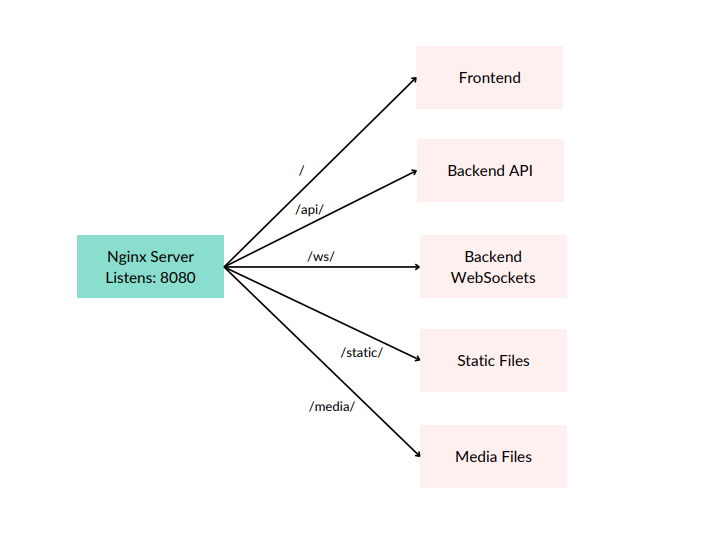
\includegraphics[width=0.6\textwidth]{figs/nginx-conf.png} 
%    \caption{Nginx Load Balancing}
%    \label{fig:nginx-conf}
%\end{figure}

\section{Monitoring and Visualization}
\subsection{Metrics Collection with Prometheus}
Prometheus \cite{rfc56} is an open-source systems monitoring and alerting toolkit designed primarily for reliability and scalability.
It works by scraping metrics from applications, storing this data in a time-series database, and allowing 
powerful queries and visualizations through its flexible query language.

It collects metrics data through a "scraping" process. This involves periodically querying an endpoint on 
the application that exposes metrics, \textit{/metrics/}. The application has been instrumented with 
django\_prometheus to provide these metrics.

Prometheus is launched using Docker and configured via \textit{prometheus.yml} file, exposing Prometheus 
on port 9090.


\subsection{Visualization using Grafana}
Grafana \cite{rfc55} is an open-source analytics and interactive visualization web application. It is highly extensible and 
provides tools to build dashboards for visualizing data from various sources, including Prometheus. Grafana supports 
a wide range of chart types and is used to create real-time, dynamic dashboards that help monitor and analyze system 
performance.

Grafana is crucial for interpreting the raw data collected by Prometheus. It connects to Prometheus, queries its 
time-series database, and presents the data in an accessible, visual format.

Grafana was deployed using Docker and configured to run on port 3001, depending on Prometheus being available 
to function correctly.

A dashboard was created featuring several metrics, as exemplified in figure \ref{fig:grafana-dashboard}. This allows for 
a comprehensive understanding of the application's behavior, facilitating detailed performance analysis and issue 
detection.

\begin{figure}[h]
    \centering 
    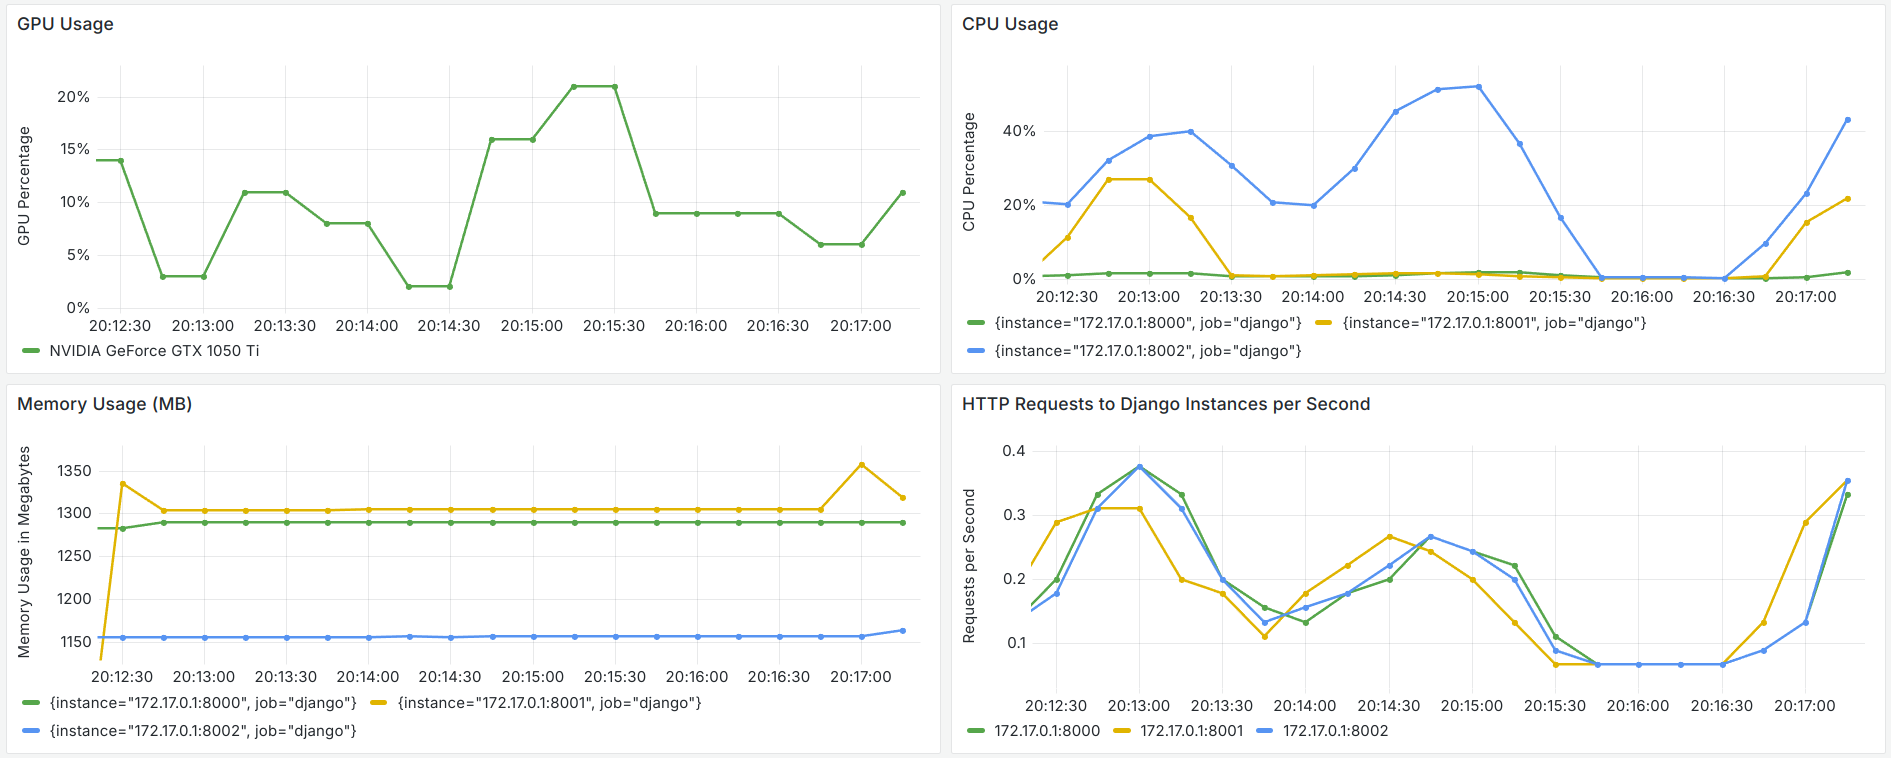
\includegraphics[width=\textwidth]{figs/grafana-dashboard2.png} 
    \caption{Grafana Dashboard}
    \label{fig:grafana-dashboard}
\end{figure}

\section{Implementation Challenges}
Implementing real-time weapon analysis for surveillance systems presents a series of significant challenges, 
primarily centered on balancing the trade-offs between speed, resolution, and system resources.

One of the difficulties arises from the key requirement to analyze and stream video content with minimal delay. 
Real-time processing is essential for effective surveillance, allowing for immediate response to potential security 
incidents as they occur. However, achieving this level of promptness often necessitates compromises in other aspects 
of the system.

A critical compromise involves the resolution of the video footage. To facilitate faster processing and streaming, 
it is often necessary to reduce the resolution of the video. This reduction speeds up the analysis by reducing the 
data load on the system, thus minimizing the delay in video streaming. However, lower resolution images can significantly 
degrade the quality of the surveillance footage.

Furthermore, the scalability of real-time video analysis systems is another major challenge, particularly when multiple 
cameras are integrated into the surveillance network. As the number of cameras increases, so too does the overload on the 
system's computational resources, including CPU and \ac{gpu} capacities. This escalation can lead to slower processing times 
and increased delays in video analysis and streaming, thereby compromising the real-time capability of the system.
%\subsection{Synchronization Issues}
\section{Scalability and Performance Optimizations}
To ensure the system can handle increasing workloads and deliver optimal performance, several 
scalability and performance optimizations were implemented across all components.

In the frontend, Web Workers were utilized to handle frame processing in the background, offloading intensive 
tasks from the main thread and keeping the user interface responsive and fluid.
Additionally, the number of DOM updates in canvas components was reduced by batching multiple updates and limiting 
unnecessary interactions with the DOM. This approach achieved smoother rendering and improved visual performance.
By managing state effectively, unnecessary calls to external services were minimized. For example, instead of making 
multiple calls to RabbitMQ, a single persistent connection was established.

On the backend, a dedicated worker pool was employed to handle frame processing in parallel. This setup took 
advantage of multi-core processors, distributing the workload among multiple workers and significantly increasing 
the system's throughput and scalability. Unused memory was periodically cleared to prevent memory leaks and maintain 
efficient memory usage.
The frequency of frames analyzed by the object detection algorithm was reduced, processing every 10th frame 
instead of every frame to balance performance with accuracy and reduce computational demands without significantly 
compromising detection capabilities.
Batch processing for frames was also implemented, allowing multiple frames to be processed simultaneously rather 
than individually, thus maximizing the \ac{gpu}'s parallel processing power.

For RabbitMQ various settings were optimized to achieve better performance. The prefetch count was increased to 
allow RabbitMQ to send more messages to consumers without waiting for acknowledgments, reducing latency and improving 
throughput.
